\documentclass[]{usiinfbachelorproject}

\captionsetup{labelfont={bf}}

\author{Andrea Vicari}

\title{Smart--IVC}
\subtitle{Cities Becoming Alive}
\versiondate{\today}
\begin{committee}
%With more than 1 advisor an error is raised...: only 1 advisor is allowed!
\advisor[Universit\`a della Svizzera Italiana, Switzerland]{Prof.}{Michele}{Lanza}
%You can comment out  these lines if you don't have any assistant
\assistant[Universit\`a della Svizzera Italiana, Switzerland]{Prof. Dr.}{Andrea}{Mocci}
\end{committee}
\newcommand{\applicationName}{Smart-IVC}


\abstract {
%The purpose of this Bachelor Project is to create a web application that provides a 3D-visualization a city and let the user interact with the entities inside it.\\
Web users have to aggregate different data from various sources whenever they are looking for some information on the Internet. Think about the student who is looking for a rented room near her university: she firstly uses a specific website to find the advertisement of a room for rent, she then looks for the address on another website that provides a map service to see if the house is located where she desires.\\

No such service exists that provides a unique environment in which the user can both visualize a city and interact with its elements. The only technologies available are either not exhaustive or too complex to use.\\

This thesis introduces Smart--IVC a web application that provides an intuitive interface and prevents the user from jumping from website to website. Through the form of a 3D-environment, this application provides an interactive visualisation of cities in which the user can directly “communicate” with the elements, executing queries on them. After having clicked on a building in the map, the user is able to get information (coordinates, address, floors etc.) about that construction and also find out what are the various relations between that specific building and the other entities in the city.\\

Smart--IVC is an application accessible by everyone and that aims to enhance the city visualisation, getting closer to the user needs.
}


\begin{document}
\maketitle

%%%%%%%%%%%%%%%%%%%%%%%%%
\section{Introduction} \label{introduction}
%%%%%%%%%%%%%%%%%%%%%%%%%
Cities nowadays are in constant evolution. They change their structure overtime through the appearance of new elements and the disappearance of old ones, thus they are very unstable and prone to changes. Important changes, might be considered with regard to the deployment and management of all types of infrastructures within cities.

Moreover, cities have a very large impact on the economic and social development of nations: they represent the real foundation where people live, where companies have their business and in which numerous services are provided. Often, a city overview is not available, so decision may be taken without having a big picture of the surrounding environment. This could lead to choices that might have a negative impact on the current city, reducing the efficiency and the life quality of the citizens.\\

To control these changes, a visualization, which provides a city overview, is required. Such a visualization is considered to be the first step towards what it is called a Smart City. A Smart City can be defined as a city which uses information and communication technologies so that its critical infrastructure as well as its components and public services provided are more interactive, efficient and so that citizens can be made more aware of them.\\
\subsection{Structure of the document}
\begin{itemize}
	\item {\bf Chapter 2}
	\item {\bf Chapter 3}
	\item {\bf Chapter 4}
	\item {\bf Chapter 5}
	\item {\bf Chapter 6}
\end{itemize}

%%%%%%%%%%%%%%%%%%%%%%%%%
\section{State of the Art} \label{stateOfTheArt}
%%%%%%%%%%%%%%%%%%%%%%%%%
The uniqueness of \applicationName resides on the fact that it provides not only a visualization of a city but, above all, it gives the possibility to the user to interact with the city itself through a simple system of visual queries.
Before getting into the details with \applicationName, the current state of city visualization must be clarified.

\subsection{Cesiumjs}
Cesium is an open-source JavaScript library for world-class 3D globes and maps that is used to create a web-based globe and map for visualizing dynamic data. 
\begin{figure} [H]
\centering
\includegraphics[width=0.8\textwidth]{images/cesium_logo}
\caption{Cesium logo}
\label{fig:cesium_logo}
\end{figure}
\begin{figure} [H]
\centering
\includegraphics[width=0.8\textwidth]{images/NewYorkCityCesium3dTiles}
\caption{An example showing a 3D visualization of the city of New York. Using Cesium 3D Tiles Tecnhology}
\label{fig:NewYorkCityCesium3dTiles}
\end{figure}
\subsection{Swiss Geospatial Portal Using 3D Tiles}
\begin{figure} [H]
\centering
\includegraphics[width=0.9\textwidth]{images/BernCitySwissTopo}
\caption{A 3D visualization of the city of Bern in the Swiss Geospatial Portal. Using Cesium 3D Tiles Tecnhology}
\label{fig:BernCitySwissTopo}
\end{figure}



%%%%%%%%%%%%%%%%%%%%%%%%%
\section{Project requirements and analysis} \label{projectRequirementsAndAnalysis}
%%%%%%%%%%%%%%%%%%%%%%%%%

%%%%%%%%%%%%%%%%%%%%%%%%%
\section{\applicationName} \label{projectDesign}
%%%%%%%%%%%%%%%%%%%%%%%%%

%%%%%%%%%%%%%%%%%%%%%%%%%
\section{Use Cases} \label{tests}
%%%%%%%%%%%%%%%%%%%%%%%%%

%%%%%%%%%%%%%%%%%%%%%%%%%
\section{Conclusions and future work or possible developments} \label{conclusions}
%%%%%%%%%%%%%%%%%%%%%%%%%


%\begin{figure} [h]
%\centering
%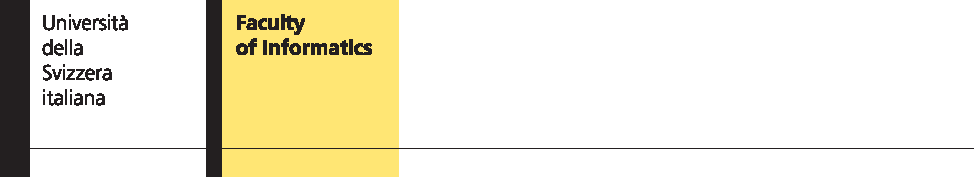
\includegraphics[width=0.5\textwidth]{logo-info.pdf}
%\caption{Caption of the figure}
%\label{fig:USILogo}
%\end{figure}

%\begin{table}[h]
%\centering
%\scalebox {0.8} {
%\begin{normalsize}\begin{tabular}{l|lll}
%\textbf{Col 1} & \textbf{Col 2} & \textbf{Col 3} & \textbf{Col 4}\\
%\hline
%1 & 2 & 3 & Goofy\\
%4 & 5 & 6 & Mickey
%\end{tabular}
%\end{normalsize}
%}
%\caption{Caption of the table}
%\label{tab:numbers}
%\end{table}

%\cite{Stru1899a}
%%%%%
\bibliographystyle{abbrv}
\bibliography{references}

\end{document}